\documentclass[a4paper,xelatex,ja=standard]{bxjsarticle}
\usepackage[dvipdfmx]{graphicx}
\usepackage[T1]{fontenc}
\usepackage{newpxtext, newpxmath}
\usepackage{verbatim}
\makeatletter

\begin{document}
\section{4次元変文データ同化}
\subsection{Cost Function}
データ同化の定式化にあたり,コスト関数を
\begin{equation}
    \label{eq:cost_function}
    \mathcal{J}(\mathbf{v}, \mathbf{v}^{0}, \mathbf{V}) = \mathcal{D}(\mathbf{v}) + \mathcal{R}(\mathbf{v}^{0}, \mathbf{V})
\end{equation}
と定義する.ここで,右辺第1項は,計測速度とCFD速度の誤差を表し
\begin{equation}
    \label{eq:error_function}
    \mathcal{D}(\mathbf{v}) = 
    \frac{\alpha}{2} \sum_{n=1}^{N} \sum_{m=1}^{M} \left\|\mathbf{v}_\text{CFD}-\mathbf{v}_{\text{MRI}}\right\|^2 \Delta x_{\mathrm{m}} \Delta y_{\mathrm{m}} \Delta z_{\mathrm{m}} \Delta t_{\mathrm{m}} 
\end{equation}
である.また,右辺第2項は,正則化項を表し
\begin{equation}
    \label{eq:regularization}
    \begin{aligned}
    \mathcal{R}(\mathbf{v}^0, \mathbf{V}) 
    &= \frac{\beta}{2} \sum_{k=1}^{M} \int_{\Gamma_\mathrm{I}} \big( \left|\mathbf{V}\right|^2+\left|\partial_s \mathbf{V}\right|^2+\left|\dot{\mathbf{V}}\right|^2+\left|\partial_s \dot{\mathbf{V}}\right|^2 \big) \, \mathrm{d}\Gamma
    + \frac{\gamma}{2} \int_{\Omega}  \big( \left|\mathbf{v}^{0}\right|^2+\left|\partial_s \mathbf{v}^{0} \right|^2  \big) \, \mathrm{d}\Omega
    \end{aligned}
\end{equation}
である.
\subsection{Discretise-Then-Optimise Approach}
流体の離散支配方程式を,ナビエ・ストークス方程式と連続の式を用いて
\begin{equation}
    \label{eq:navier-stokes}
    \frac{\mathbf{v}^{k+1}-\mathbf{v}^k}{\Delta t_{\text{CFD}}} + \left( \frac{3}{2}\mathbf{v}^k - \frac{1}{2}\mathbf{v}^{k-1} \right) \cdot \nabla \mathbf{v}^{k+1 / 2} + \frac{1}{\rho} \nabla p^{k+1} - \nu \nabla^2 \mathbf{v}^{k+1/2} + \mathbf{K}(\phi) \mathbf{v}^{k+1/2} = \mathbf{0}
\end{equation}
\begin{equation}
    \label{eq:continuity}
    \nabla \cdot \mathbf{v}^{k+1}=\mathbf{0}
\end{equation}
と記述する.ここで,移流項に対し2次精度Adams-Bashforth法,拡散項に対してはCrank-Nicolson法を用いた.
式(\ref{eq:navier-stokes}),式(\ref{eq:continuity})に対し,重み付き残差法による弱形式を導き,全CFD時間ステップで総和を取ると,拘束条件が
\begin{equation}
    \label{eq:weak-form}
    \mathcal{F}=\sum_{k=0}^{N-1} \mathcal{F}_{k} = 0
\end{equation}
と表せる.ここで,
\begin{equation}
    \label{eq:weak-form-k}
    \begin{aligned}
        \mathcal{F}_{k} & = \int_{\Omega} \mathbf{w}^{k+1} \cdot \bigg( \frac{\mathbf{v}^{k+1}-\mathbf{v}^k}{\Delta t_{\text{CFD}}} +\left( \frac{3}{2}\mathbf{v}^k - \frac{1}{2}\mathbf{v}^{k-1} \right) \cdot \nabla \mathbf{v}^{k+1 / 2} + \frac{1}{\rho} \nabla p^{k+1} - \nu \nabla^2 \mathbf{v}^{k+1/2} + \mathbf{K}(\phi) \mathbf{v}^{k+1/2} \bigg) \, \mathrm{d}\Omega \\
        &+ \int_{\Omega} q^{k+1}(\nabla \cdot \mathbf{v}^{k+1}) \, \mathrm{d}\Omega - \int_{\Gamma_1} \lambda^{k+1} \cdot (\mathbf{v}^{k+1} - \mathbf{V}^{k+1}) \, \mathrm{d}\Gamma - \int_{\Gamma_1} \boldsymbol{\eta}^{k+1} \cdot \mathbf{w}^{k+1} \, \mathrm{d}\Gamma = 0
    \end{aligned}
\end{equation}
である.数値安定化手法に,SUPG/PSPG法を用いたが,煩雑を避け,これらの項は省略する.さらに,目的関数・拘束条件を合わせたLagrange関数
\begin{equation}
    \label{eq:lagrange}
    \mathcal{L} = \mathcal{F} + \mathcal{J}
\end{equation}
より,制約なし最小化問題を
\begin{equation}
    \label{eq:minimization}
    \min_{\mathbf{v}^{0}, \mathbf{V}} \mathcal{L}
\end{equation}
と定義する.

主問題は,
\begin{equation}
    \everymath{\displaystyle}
    \setlength{\arraycolsep}{0.5pt}
    \renewcommand{\arraystretch}{2.5}
    \label{eq:main_problem}
    {}^{t}\!\left\langle\frac{\partial \mathcal{L}}{\partial \mathbf{w}}, \tilde{\mathbf{w}}\right\rangle
    = \begin{pmatrix}
        \left\langle\frac{\partial \mathcal{L}}{\partial \mathbf{w}^{\scriptscriptstyle 1}}, \tilde{\mathbf{w}}^{\scriptscriptstyle 1}\right\rangle \\
        \vdots \\
        \left\langle\frac{\partial \mathcal{L}}{\partial \mathbf{w}^{\scriptscriptstyle N}}, \tilde{\mathbf{w}}^{\scriptscriptstyle N}\right\rangle 
    \end{pmatrix}
    =\mathbf{0}
    ,\quad
    {}^{t}\!\left\langle\frac{\partial \mathcal{L}}{\partial q}, \tilde{q}\right\rangle
    = \begin{pmatrix}
        \left\langle\frac{\partial \mathcal{L}}{\partial q^{\scriptscriptstyle 1}}, \tilde{q}^{\scriptscriptstyle 1}\right\rangle \\
        \vdots \\
        \left\langle\frac{\partial \mathcal{L}}{\partial q^{\scriptscriptstyle N}}, \tilde{q}^{\scriptscriptstyle N}\right\rangle 
    \end{pmatrix}
    =\mathbf{0}
    ,\quad
    {}^{t}\!\left\langle\frac{\partial \mathcal{L}}{\partial \boldsymbol{\lambda}}, \tilde{\boldsymbol{\lambda}}\right\rangle
    = \begin{pmatrix}
        \left\langle\frac{\partial \mathcal{L}}{\partial \boldsymbol{\lambda}^{\scriptscriptstyle 1}}, \tilde{\boldsymbol{\lambda}}^{\scriptscriptstyle 1}\right\rangle \\
        \vdots \\
        \left\langle\frac{\partial \mathcal{L}}{\partial \boldsymbol{\lambda}^{\scriptscriptstyle N}}, \tilde{\boldsymbol{\lambda}}^{\scriptscriptstyle N}\right\rangle 
    \end{pmatrix}
    =\mathbf{0}
\end{equation}
と表され,各時間ステップ$k \ (1 \leq k \leq N)$において
\begin{align}
    &\begin{aligned}
        \label{eq:foward_w}
        \left\langle\frac{\partial \mathcal{L}}{\partial \mathbf{w}^k}, \tilde{\mathbf{w}}^k\right\rangle
        & = \int_{\Omega} \bigg( \tilde{\mathbf{w}}^{k+1} \cdot \frac{\mathbf{v}^{k+1}-\mathbf{v}^k}{\Delta t_{\text{CFD}}}
        +\tilde{\mathbf{w}}^{k+1} \cdot \left( \frac{3}{2}\mathbf{v}^k - \frac{1}{2}\mathbf{v}^{k-1} \right) \cdot \nabla \mathbf{v}^{k+1 / 2} 
        + \frac{1}{\rho} p^{k+1} (\nabla \cdot \tilde{\mathbf{w}}^{k}) \\
        &- \nu \nabla \tilde{\mathbf{w}}^{k+1} : \mathbf{v}^{k+1/2} + \tilde{\mathbf{w}}^{k+1} \cdot \mathbf{K}(\phi) \mathbf{v}^{k+1/2} \bigg) \, \mathrm{d}\Omega
        - \int_{\Gamma_1} \boldsymbol{\eta}^{k+1} \cdot \tilde{\mathbf{w}}^{k+1} \, \mathrm{d}\Gamma = 0
    \end{aligned} \\
    \label{eq:foward_q} 
    & \left\langle\frac{\partial \mathcal{L}}{\partial q^k}, \tilde{q}^k\right\rangle
    =\int_{\Omega} \tilde{q}^k(\nabla \cdot \mathbf{v}^{k+1}) \, \mathrm{d}\Omega
    = 0 \\
    \label{eq:foward_lambda} 
    &\left\langle\frac{\partial \mathcal{L}}{\partial \boldsymbol{\lambda}^k}, \tilde{\boldsymbol{\lambda}}^k\right\rangle
    = \int_{\Gamma_1} \tilde{\boldsymbol{\lambda}}^k \cdot (\mathbf{v}^{k+1} - \mathbf{V}^{k+1}) \, \mathrm{d}\Gamma
    = 0
\end{align}
とそれぞれ記述できる.

次に,随伴問題は,
\begin{equation}
    \everymath{\displaystyle}
    \setlength{\arraycolsep}{0.5pt}
    \renewcommand{\arraystretch}{2.5}
    \label{eq:adjoint_problem}
    {}^{t}\!\left\langle\frac{\partial \mathcal{L}}{\partial \mathbf{v}}, \tilde{\mathbf{v}}\right\rangle
    = \begin{pmatrix}
        \left\langle\frac{\partial \mathcal{L}}{\partial \mathbf{v}^{\scriptscriptstyle 1}}, \tilde{\mathbf{v}}^{\scriptscriptstyle 1}\right\rangle \\
        \vdots \\
        \left\langle\frac{\partial \mathcal{L}}{\partial \mathbf{v}^{\scriptscriptstyle N}}, \tilde{\mathbf{v}}^{\scriptscriptstyle N}\right\rangle 
    \end{pmatrix}
    =\mathbf{0}
    ,\quad
    {}^{t}\!\left\langle\frac{\partial \mathcal{L}}{\partial p}, \tilde{p}\right\rangle
    = \begin{pmatrix}
        \left\langle\frac{\partial \mathcal{L}}{\partial p^{\scriptscriptstyle 1}}, \tilde{p}^{\scriptscriptstyle 1}\right\rangle \\
        \vdots \\
        \left\langle\frac{\partial \mathcal{L}}{\partial p^{\scriptscriptstyle N}}, \tilde{p}^{\scriptscriptstyle N}\right\rangle 
    \end{pmatrix}
    =\mathbf{0}
    ,\quad
    {}^{t}\!\left\langle\frac{\partial \mathcal{L}}{\partial \boldsymbol{\eta}}, \tilde{\boldsymbol{\eta}}\right\rangle
    = \begin{pmatrix}
        \left\langle\frac{\partial \mathcal{L}}{\partial \boldsymbol{\eta}^{\scriptscriptstyle 1}}, \tilde{\boldsymbol{\eta}}^{\scriptscriptstyle 1}\right\rangle \\
        \vdots \\
        \left\langle\frac{\partial \mathcal{L}}{\partial \boldsymbol{\eta}^{\scriptscriptstyle N}}, \tilde{\boldsymbol{\eta}}^{\scriptscriptstyle N}\right\rangle 
    \end{pmatrix}
    =\mathbf{0}
\end{equation}
と表され,各時間ステップ$k \ (1 \leq k \leq N)$において
\begin{align}
    &\begin{aligned}
        \label{eq:adjoint_v}
        \left\langle\frac{\partial \mathcal{L}}{\partial \mathbf{v}^k}, \tilde{\mathbf{v}}^k\right\rangle
        = &\int_{\Omega} \bigg( \frac{\mathbf{w}^{k} - \mathbf{w}^{k+1}}{\Delta t_{\text{CFD}}} \cdot \tilde{\mathbf{v}}^k
        + \frac{1}{4} \mathbf{w}^{k} \cdot \left( 3\mathbf{v}^{k-1} - \mathbf{v}^{k-2} \right) \cdot \nabla \tilde{\mathbf{v}}^{k}
        + \frac{3}{4} \mathbf{w}^{k+1} \cdot \tilde{\mathbf{v}}^k \cdot \nabla \mathbf{v}^{k+1} \\ 
        &+ \frac{1}{4} \mathbf{w}^{k+1} \cdot \left( 3\mathbf{v}^k - \mathbf{v}^{k-1} \right) \cdot \nabla \tilde{\mathbf{v}}^{k}
        - \frac{1}{4} \mathbf{w}^{k+2} \cdot \tilde{\mathbf{v}}^{k} \cdot \nabla \mathbf{v}^{k+1} 
        - \frac{1}{4}  \mathbf{w}^{k+2} \cdot \tilde{\mathbf{v}}^{k} \cdot \nabla \mathbf{v}^{k} \\
        & +  q^{k+1} (\nabla \cdot \tilde{\mathbf{v}}^{k+1})
        - \frac{1}{2} \nu \left(\nabla \mathbf{w}^{k} + \nabla \mathbf{w}^{k+1}\right) : \nabla \tilde{\mathbf{v}}^k
        + \frac{1}{2} \left(\mathbf{w}^{k} + \mathbf{w}^{k+1}\right) \cdot \mathbf{K}(\phi) \tilde{\mathbf{v}}^k 
        \bigg) \, \mathrm{d}\Omega \\
        &+ \int_{\Gamma_1} \lambda^{k+1} \cdot \tilde{\mathbf{v}}^{k} \, \mathrm{d}\Gamma
        + \alpha \smash{\sum_{i, j, k=1}^{M}} \left(\mathbf{v}_\text{c}-\mathbf{v}_{\text{m}}\right) \tilde{\mathbf{v}} \Delta x_{\mathrm{m}} \Delta y_{\mathrm{m}} \Delta z_{\mathrm{m}} \Delta t_{\mathrm{m}}
        = 0
    \end{aligned} \\
    \label{eq:adjoint_p} 
    & \left\langle\frac{\partial \mathcal{L}}{\partial p^k}, \tilde{p}^k\right\rangle
    =\int_{\Omega} \tilde{p}^k(\nabla \cdot \mathbf{w}^{k}) \, \mathrm{d}\Omega 
    = 0 \\
    \label{eq:adjoint_eta} 
    &\left\langle\frac{\partial \mathcal{L}}{\partial \boldsymbol{\eta}^k}, \tilde{\boldsymbol{\eta}}^k\right\rangle
    =\int_{\Gamma_1} \tilde{\boldsymbol{\eta}}^k \cdot \mathbf{w}^k \, \mathrm{d}\Omega 
    = 0
\end{align}
とそれぞれ記述できる(Appendix A).ここで,式(\ref{eq:adjoint_v})に関し
\begin{equation}
    \begin{cases}
        \displaystyle \mathbf{v}^{k-2} = \mathbf{v}^{0} & \text{for } k=1 \\
        \displaystyle \mathbf{w}^{k+2} = \mathbf{0} & \text{for } k=N-1 \\
        \displaystyle \mathbf{w}^{k+1} = \mathbf{w}^{k+2} = \mathbf{0} & \text{for } k=N
    \end{cases}
\end{equation}
である.

最後に,主問題,随伴問題より得た変数から,初期条件と,各時間ステップ$k \ (1 \leq k \leq N)$における入口速度境界条件の感度
\begin{align}
    \label{eq:adjoint_v0}
    &\begin{aligned}
        \left\langle\frac{\partial \mathcal{L}}{\partial \mathbf{v}^0}, \tilde{\mathbf{v}}^0\right\rangle
        = &\int_{\Omega} \bigg(- \frac{ \mathbf{w}^{1}}{\Delta t_{\text{CFD}}} \cdot \tilde{\mathbf{v}}^0
        + \frac{3}{4} \mathbf{w}^{1} \cdot \tilde{\mathbf{v}}^0 \cdot \nabla \mathbf{v}^{1}
        + \frac{1}{2} \mathbf{w}^{1} \cdot \mathbf{v}^0 \cdot \nabla \tilde{\mathbf{v}}^{k} 
        - \frac{1}{4} \mathbf{w}^{2} \cdot \tilde{\mathbf{v}}^{0} \cdot \nabla \mathbf{v}^1 \\
        &- \frac{1}{4} \mathbf{w}^{2} \cdot \tilde{\mathbf{v}}^{0} \cdot \nabla \mathbf{v}^{0}
         - \frac{1}{2} \nu \nabla \mathbf{w}^{1} : \nabla \tilde{\mathbf{v}}^0
        + \frac{1}{2} \mathbf{w}^{1} \cdot \mathbf{K}(\phi) \tilde{\mathbf{v}}^0 
        \bigg) \, \mathrm{d}\Omega 
    \end{aligned} \\
    &\left\langle\frac{\partial \mathcal{L}}{\partial \mathbf{V}^k}, \widetilde{\mathbf{V}}^k\right\rangle
    =\int_{\Gamma_{\mathrm{I}}} \beta \partial_s \mathbf{V}^k \cdot \widetilde{\mathbf{V}}^k+\lambda \cdot \widetilde{\mathbf{V}}^k \mathrm{d} \Gamma
\end{align}
を導出し,これらを用いて最適性条件

\newpage
\section{数値計算例}

\begin{figure}
    \begin{center}
      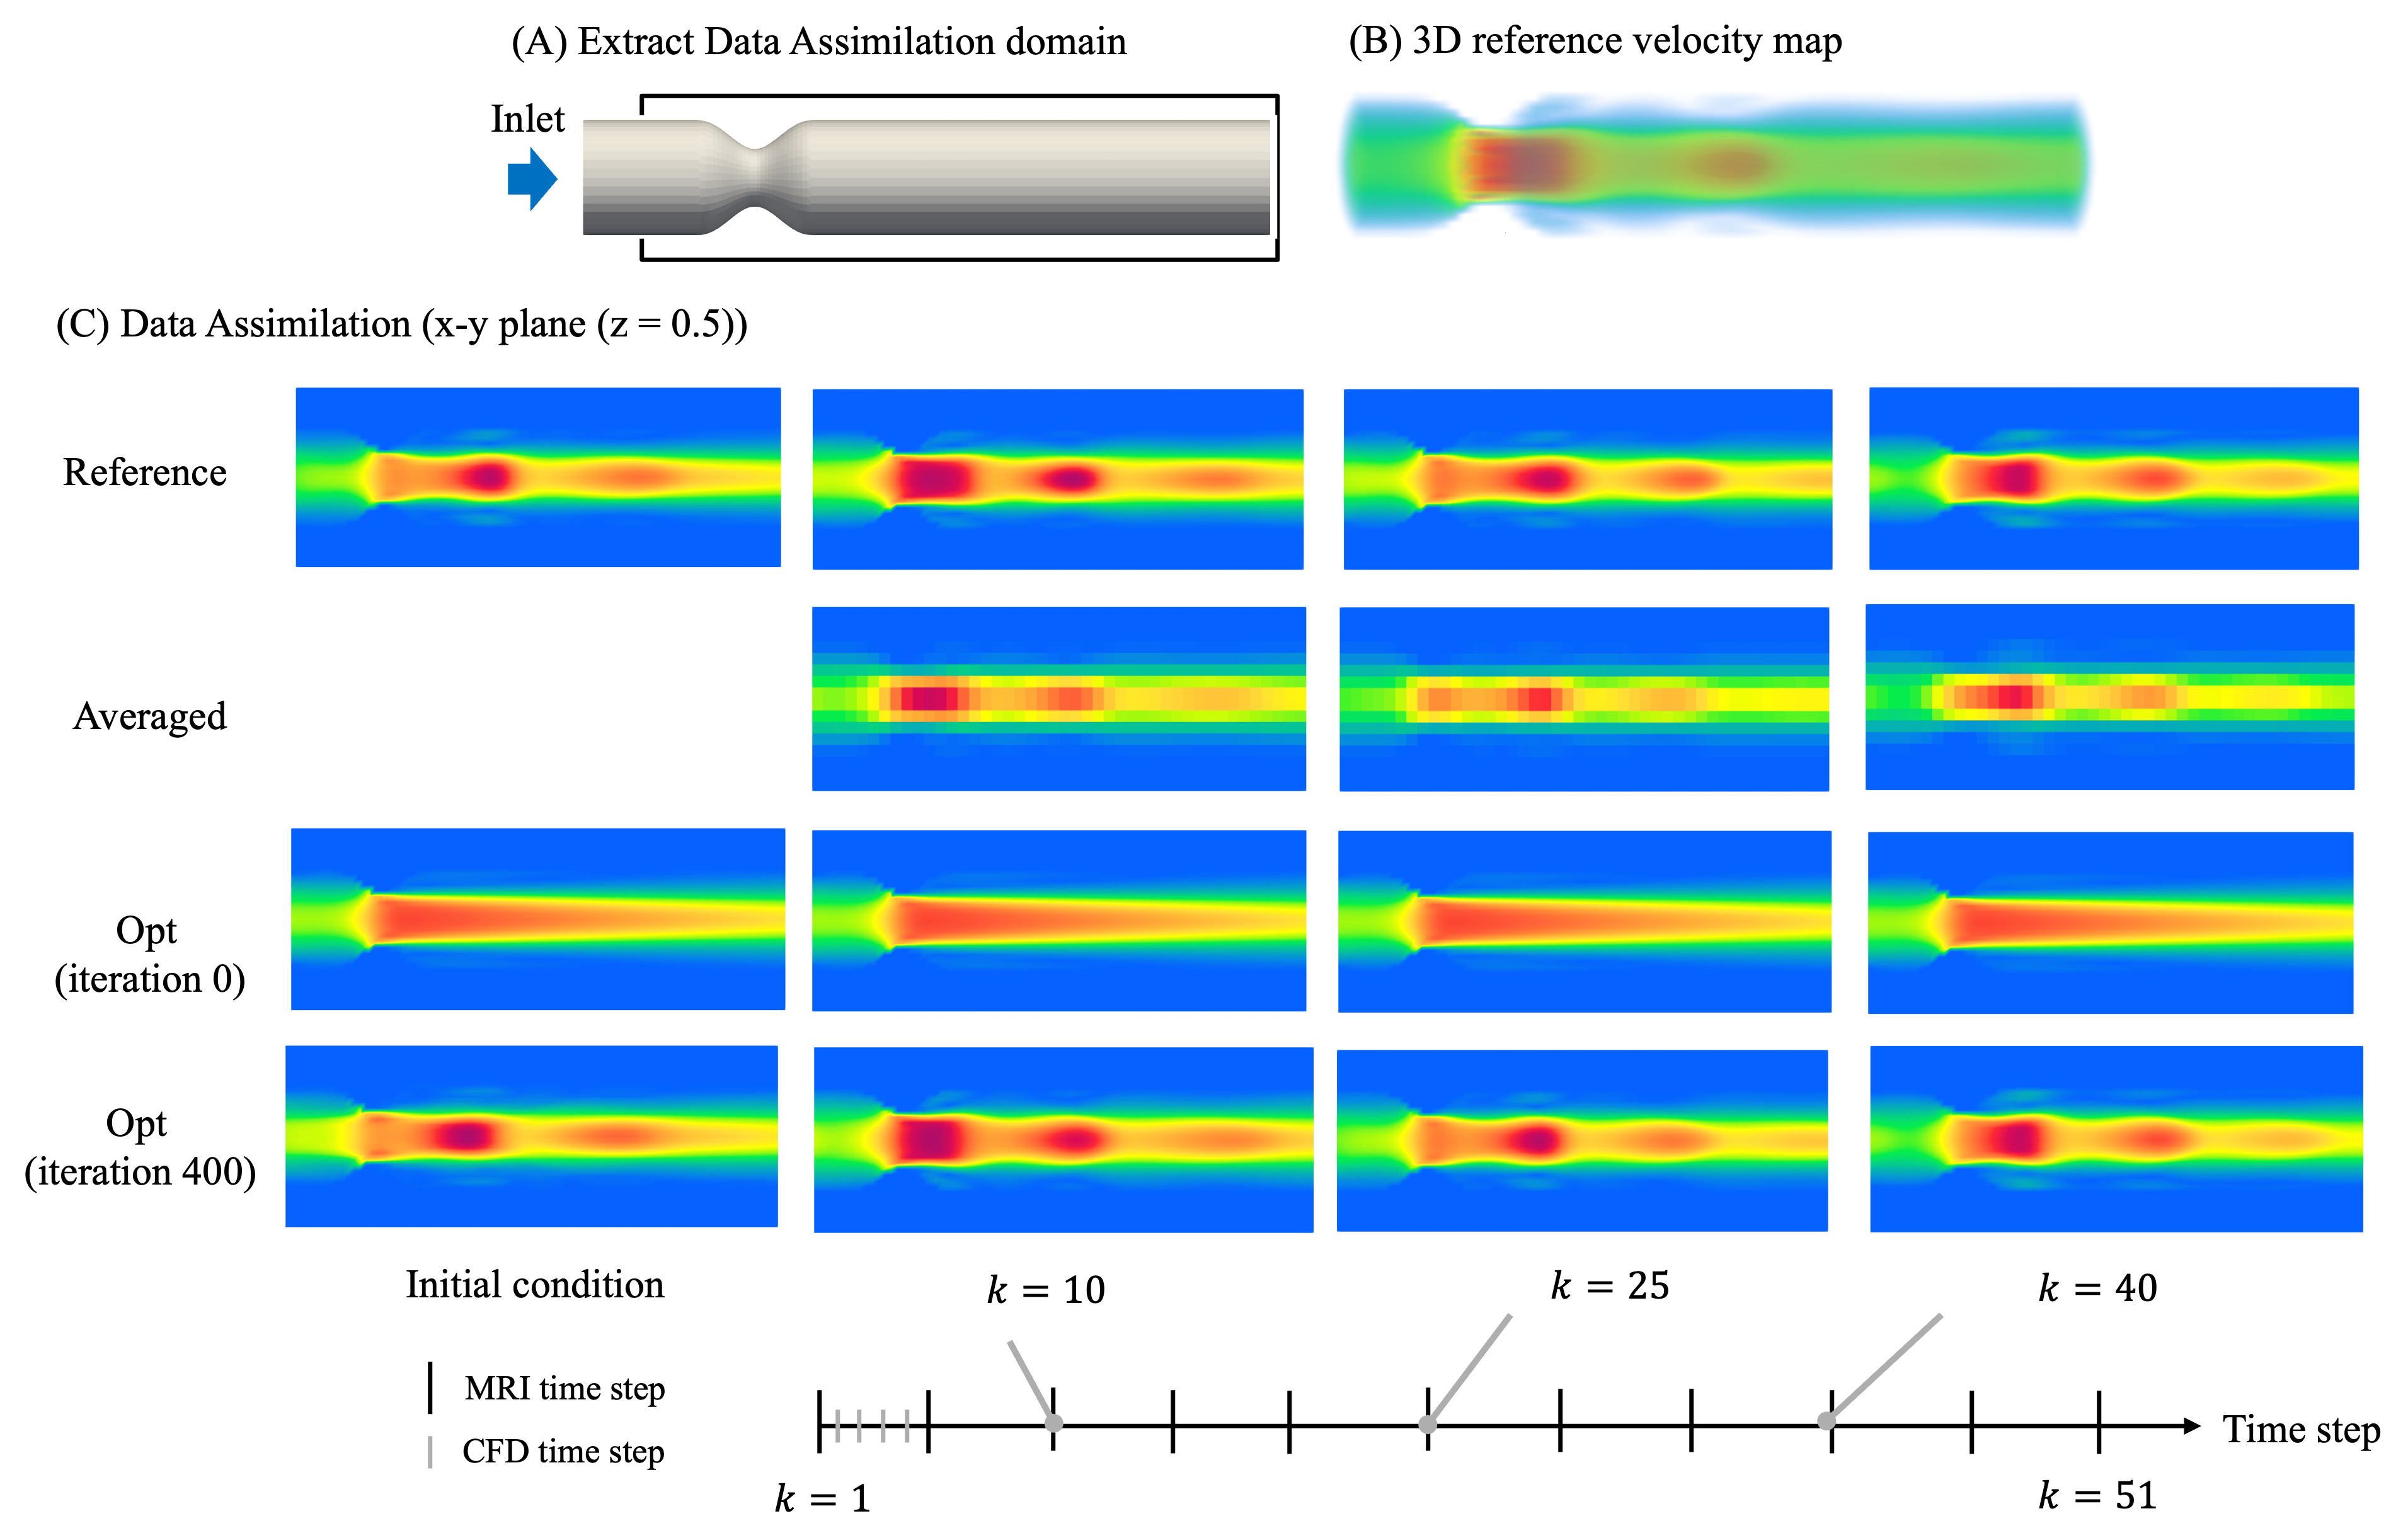
\includegraphics[scale=0.5]{figures/results_all.png} 
    \end{center}
    \caption{狭窄管流れの数値計算例.}
    \label{fig:2}    
\end{figure}

\newpage
\appendix
\renewcommand{\appendixname}{Appendix }
\section{$\mathbf{v}$に対するガトー微分}

ラグランジュ関数の$\mathbf{v}$でのガトー微分について,式(\ref{eq:adjoint_problem})のベクトルk成分は,
\begin{equation}
    \label{eq:adjoint_vdd}
    \left\langle\frac{\partial \mathcal{L}}{\partial \mathbf{v}^k}, \tilde{\mathbf{v}}^k\right\rangle
    = \begin{cases}
      \displaystyle \left\langle\frac{\partial \mathcal{J}}{\partial \mathbf{v}^{k}}, \tilde{\mathbf{v}}^{k}\right\rangle
      + \displaystyle \left\langle\frac{\partial \mathcal{F}_{k-1}}{\partial \mathbf{v}^{k}}, \tilde{\mathbf{v}}^{k}\right\rangle
      + \displaystyle \left\langle\frac{\partial \mathcal{F}_{k}}{\partial \mathbf{v}^{k}}, \tilde{\mathbf{v}}^{k}\right\rangle
      + \displaystyle \left\langle\frac{\partial \mathcal{F}_{k+1}}{\partial \mathbf{v}^{k}}, \tilde{\mathbf{v}}^{k}\right\rangle 
      & \text { for } 1 \leq k<N-1 \\[12pt]
      \displaystyle \left\langle\frac{\partial \mathcal{J}}{\partial \mathbf{v}^{k}}, \tilde{\mathbf{v}}^{k}\right\rangle
      + \displaystyle \left\langle\frac{\partial \mathcal{F}_{k-1}}{\partial \mathbf{v}^{k}}, \tilde{\mathbf{v}}^{k}\right\rangle
      + \displaystyle \left\langle\frac{\partial \mathcal{F}_{k}}{\partial \mathbf{v}^{k}}, \tilde{\mathbf{v}}^{k}\right\rangle
      & \text { for } k=N-1 \\[12pt]
      \displaystyle \left\langle\frac{\partial \mathcal{J}}{\partial \mathbf{v}^{k}}, \tilde{\mathbf{v}}^{k}\right\rangle
      + \displaystyle \left\langle\frac{\partial \mathcal{F}_{k-1}}{\partial \mathbf{v}^{k}}, \tilde{\mathbf{v}}^{k}\right\rangle
      & \text { for } k=N \\[12pt]
    \end{cases}
\end{equation}
であり,右辺はそれぞれ
\begin{align}
    &\left\langle\frac{\partial \mathcal{J}}{\partial \mathbf{v}^k}, \tilde{\mathbf{v}}^k\right\rangle
    =  \alpha \smash{\sum_{i, j, k=1}^{M}} \left(\mathbf{v}_\text{c}-\mathbf{v}_{\text{m}}\right) \tilde{\mathbf{v}} \Delta x_{\mathrm{m}} \Delta y_{\mathrm{m}} \Delta z_{\mathrm{m}} \Delta t_{\mathrm{m}} \\
    &\left\langle\frac{\partial \mathcal{F}_{k-1}}{\partial \mathbf{v}^k}, \tilde{\mathbf{v}}^k\right\rangle
    = \int_{\Omega} \bigg( \mathbf{w}^{k} \cdot \frac{\tilde{\mathbf{v}}^k}{\Delta t_{\text{CFD}}} + \frac{1}{4} \mathbf{w}^{k} \cdot \left( 3\mathbf{v}^{k-1} - \mathbf{v}^{k-2} \right) \cdot \nabla \tilde{\mathbf{v}}^{k} 
    - \frac{1}{2} \nu \nabla \mathbf{w}^{k}: \nabla \tilde{\mathbf{v}}^k + \frac{1}{2} \mathbf{w}^{k} \cdot \mathbf{K}(\phi) \tilde{\mathbf{v}}^k \bigg) \, \mathrm{d}\Omega \\
    &\begin{aligned}
        \left\langle\frac{\partial \mathcal{F}_k}{\partial \mathbf{v}^k}, \tilde{\mathbf{v}}^k\right\rangle
        &= \int_{\Omega} \bigg( \mathbf{w}^{k+1} \cdot \frac{-\tilde{\mathbf{v}}^k}{\Delta t_{\text{CFD}}} + \frac{3}{4} \mathbf{w}^{k+1} \cdot \tilde{\mathbf{v}}^k \cdot \nabla \mathbf{v}^{k+1} + \frac{1}{4} \mathbf{w}^{k+1} \cdot \left( 3\mathbf{v}^k - \mathbf{v}^{k-1} \right) \cdot \nabla \tilde{\mathbf{v}}^{k} \\
        &- \frac{1}{2} \nu \nabla \mathbf{w}^{k+1}: \nabla \tilde{\mathbf{v}}^k + \frac{1}{2} \mathbf{w}^{k+1} \cdot \mathbf{K}(\phi) \tilde{\mathbf{v}}^k \bigg) \, \mathrm{d}\Omega
    \end{aligned} \\
    &\left\langle\frac{\partial \mathcal{F}_{k+1}}{\partial \mathbf{v}^k}, \tilde{\mathbf{v}}^k\right\rangle
    = \int_{\Omega} \bigg( - \frac{1}{4}\mathbf{w}^{k+2} \cdot \tilde{\mathbf{v}}^{k} \cdot \nabla \mathbf{v}^{k+1} 
    - \frac{1}{4} \mathbf{w}^{k+2} \cdot \tilde{\mathbf{v}}^{k} \cdot \nabla \mathbf{v}^{k}\bigg) \, \mathrm{d}\Omega 
\end{align}
と表せる.

\end{document}
